\chapter{Исследовательская часть}

\section{Постановка исследования}

Предметом исследования является влияние применения различных типов индексов в базе данных на время выполнения запросов к базе данных.

В исследовании задействованы следующие типы индексов \cite{pg-indexes}:

\begin{enumerate}
	\item BTREE -- механизм работы данного индекса построен на B-дереве. Используются для увеличения скорости работы запросов, использующих операторы сравнения;
	\item HASH -- такие индексы хранят хэш-код, полученный из значения индексированного столбца. Используются только для запросов, с оператором сравнения на равенство;
	\item GIN -- эффективны для запросов, в которых используются компонентные значения, такие как массивы.
\end{enumerate}

\section{Технические характеристики}

Приведены технические характеристики устройства, на котором производилось исследование:

\begin{itemize}[label=—]
	\item Процессор 11th Gen Intel(R) Core(TM) i7-11370H @ 3.30 Ггц;
	\item 4 физических и 8 логических ядер;
	\item Оперативная память 16 ГБайт;
	\item Система Windows 11 Home.
\end{itemize}

Исследование проводилось на ноутбуке. Во время исследования устройство было подключено к питанию,
все фоновые процессы были завершены.

\section{План исследования}

В процессе исследования последовательно выполнялись запросы к базе данных. Для каждой размерности таблицы из
списка [200, 500, 1000, 2000, 5000, 10000, 25000, 50000, 75000, 100000, 200000, 300000, 400000, 500000] проводилось по 10
замеров, далее считалось среднее время выполнения. Замер времени выполнения каждого запроса осуществлялся с помощью 
конструкции EXPLAIN ANALYZE \cite{pg-explain}. Перед началом тестирования было выключено параллельное выполнение запросов. 
Сами запросы осуществлялись на таблицах StandartTraining -- основная таблица базы данных со множеством полей, для которой создавались индексы и 
StandartTraining\_noindex -- её копией, без использования индексов. Для каждого теста таблицы заполнялись тестовыми данными.
Также, после каждого замера проводилась очистка таблиц, и очищались устаревшие кортежи с помощью конструкции VACUUM ANALYZE \cite{pg-vacuum}. 

В листинге \ref{lst:create_indexes} приведено создание индексов базы данных. BTREE индекс создаётся на колонку названия мероприятия,
HASH создаётся на поле даты и времени, GIN создаётся на массив идентификаторов тренера и спортивного пространства.

\lstinputlisting[
    language=SQL,
    caption={Создание индексов},
    label=lst:create_indexes,
    frame=single 
]{listings/create_indexes.sql}



В листингах \ref{lst:sql_with_BTREE}, \ref{lst:sql_with_HASH}, \ref{lst:sql_with_GIN} приведены тестовые запросы, использующие BTREE, HASH, GIN индексы соответственно.

\lstinputlisting[
    caption={Запрос с использованием BTREE-индекса},
    label=lst:sql_with_BTREE,
    frame=single 
]{listings/BTree_index.sql}

\lstinputlisting[
    caption={Запрос с использованием HASH-индекса},
    label=lst:sql_with_HASH,
    frame=single 
]{listings/Hash_index.sql}

\lstinputlisting[
    caption={Запрос с использованием GIN-индекса},
    label=lst:sql_with_GIN,
    frame=single 
]{listings/Gin_index.sql}

В листингах \ref{lst:sql_without_BTREE}, \ref{lst:sql_without_HASH}, \ref{lst:sql_without_GIN} приведены тестовые запросы, эквивалентые
запросам в листингах \ref{lst:sql_with_BTREE}, \ref{lst:sql_with_HASH}, \ref{lst:sql_with_GIN} соответственно, но без использования индексов.

\lstinputlisting[
    caption={Запрос без использования BTREE-индекса},
    label=lst:sql_without_BTREE,
    frame=single 
]{listings/BTree_no_index.sql}

\lstinputlisting[
    caption={Запрос без использования HASH-индекса},
    label=lst:sql_without_HASH,
    frame=single 
]{listings/Hash_no_index.sql}

\lstinputlisting[
    caption={Запрос без использования GIN-индекса},
    label=lst:sql_without_GIN,
    frame=single 
]{listings/Gin_no_index.sql}

\section{Результаты исследования}

По результатам исследования были получены значения времени выполнения запросов, приведённые в таблицах
\ref{tab:res_btree_exe}, \ref{tab:res_hash_exe}, \ref{tab:res_gin_exe}.


\begin{table}[H]
	\centering
	\caption{Время выполнения запросов с BTREE индексом и без}
	\begin{tabular}{|p{5cm}|p{5cm}|p{5cm}|}
	\hline
	Количество записей в таблице & Без индекса(мс) & С индексом(мс) \\
	\hline
	200 & 0.0232 & 0.0199 \\
	\hline
	500 & 0.0387 & 0.0463 \\
	\hline
	1000 & 0.0638 & 0.0527 \\
	\hline
	2000 & 0.1180 & 0.0831 \\
	\hline
	5000 & 0.2762 & 0.1182 \\
	\hline
	10000 & 0.5252 & 0.2101 \\
	\hline
	25000 & 1.4927 & 0.4418 \\
	\hline
	50000 & 2.5391 & 0.9598 \\
	\hline
	75000 & 3.9915 & 1.3309 \\
	\hline
	100000 & 5.4074 & 1.7083 \\
	\hline
	200000 & 13.4504 & 3.5008 \\
	\hline
	300000 & 24.8811 & 5.3168 \\
	\hline
	400000 & 30.6230 & 7.2296 \\
	\hline
	500000 & 37.5275 & 8.5517 \\
	\hline
	\end{tabular}
	\label{tab:res_btree_exe}
\end{table}

\begin{table}[H]
	\centering
	\caption{Время выполнения запросов с HASH индексом и без}
	\begin{tabular}{|p{5cm}|p{5cm}|p{5cm}|}
	\hline
	Количество записей в таблице & Без индекса(мс) & С индексом(мс) \\
	\hline
	200 & 0.0183 & 0.0184 \\
	\hline
	500 & 0.0407 & 0.0153 \\
	\hline
	1000 & 0.0629 & 0.0145 \\
	\hline
	2000 & 0.1316 & 0.0154 \\
	\hline
	5000 & 0.2900 & 0.0135 \\
	\hline
	10000 & 0.5646 & 0.0133 \\
	\hline
	25000 & 1.3692 & 0.0168 \\
	\hline
	50000 & 2.9975 & 0.0165 \\
	\hline
	75000 & 4.3463 & 0.0146 \\
	\hline
	100000 & 5.5263 & 0.0169 \\
	\hline
	200000 & 11.3494 & 0.0228 \\
	\hline
	300000 & 41.7652 & 0.0319 \\
	\hline
	400000 & 54.2973 & 0.0309 \\
	\hline
	500000 & 47.1357 & 0.0407 \\
	\hline
	\end{tabular}
	\label{tab:res_hash_exe}
\end{table}

\begin{table}[H]
	\centering
	\caption{Время выполнения запросов с GIN индексом и без}
	\begin{tabular}{|p{5cm}|p{5cm}|p{5cm}|}
	\hline
	Количество записей в таблице & Без индекса(мс) & С индексом(мс) \\
	\hline
	200 & 0.0169 & 0.0368 \\
	\hline
	500 & 0.0337 & 0.0841 \\
	\hline
	1000 & 0.0572 & 0.0608 \\
	\hline
	2000 & 0.1075 & 0.0993 \\
	\hline
	5000 & 0.2567 & 0.2156 \\
	\hline
	10000 & 0.5087 & 0.4218 \\
	\hline
	25000 & 1.2448 & 1.0174 \\
	\hline
	50000 & 2.6809 & 2.1434 \\
	\hline
	75000 & 4.0070 & 3.2908 \\
	\hline
	100000 & 5.3215 & 4.3646 \\
	\hline
	200000 & 11.1057 & 8.8471 \\
	\hline
	300000 & 16.1611 & 13.1854 \\
	\hline
	400000 & 30.7479 & 18.0912 \\
	\hline
	500000 & 38.5459 & 21.9800 \\
	\hline
	\end{tabular}
	\label{tab:res_gin_exe}
\end{table}

На основе таблиц \ref{tab:res_btree_exe}, \ref{tab:res_hash_exe}, \ref{tab:res_gin_exe} были построены графики
\ref{fig:graph_btree_exe}, \ref{fig:graph_hash_exe}, \ref{fig:graph_gin_exe} соответственно.

\begin{figure}[H]
	\centering
	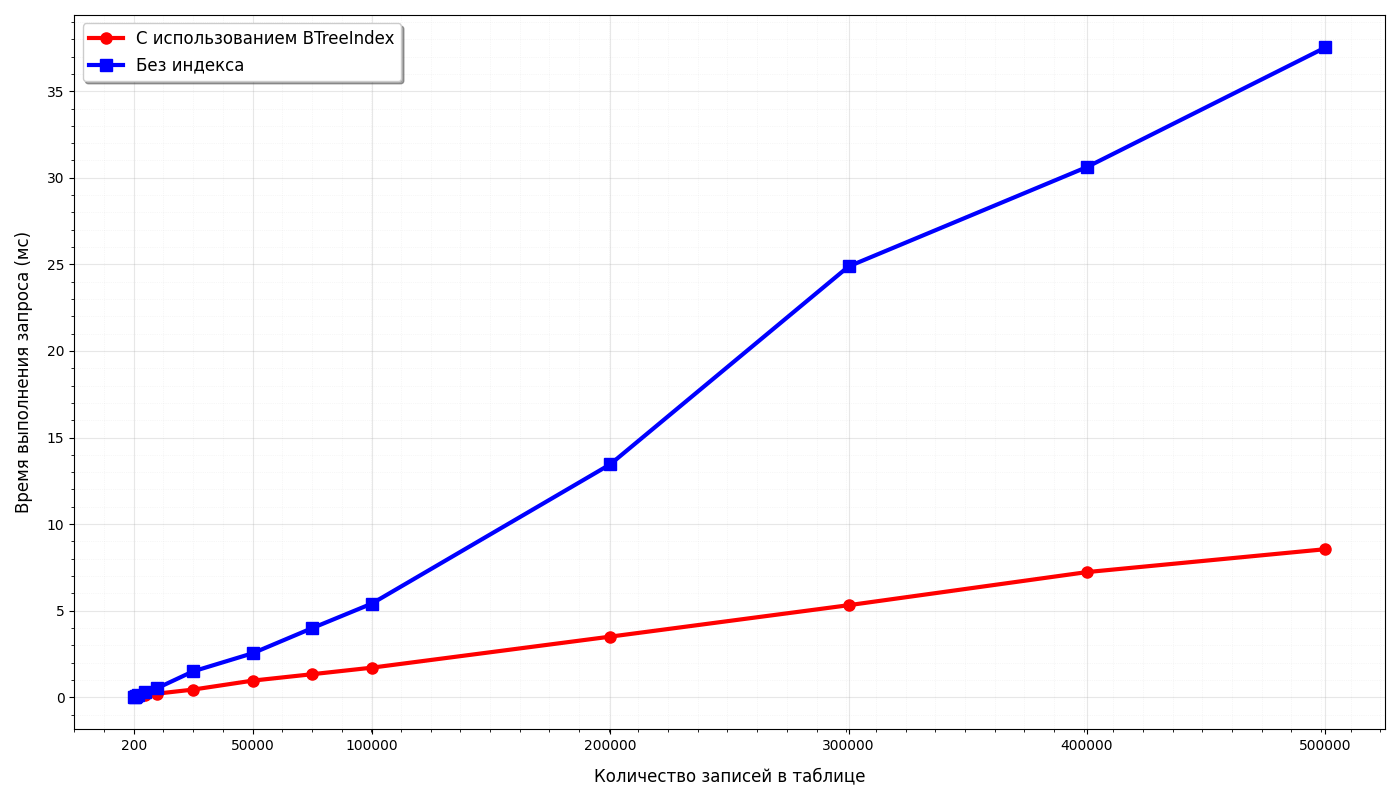
\includegraphics[width=1\textwidth]{img/btree.png}
	\caption{График времени выполнения запросов от количество записей в таблице с использованием BTREE-индекса и без него}
	\label{fig:graph_btree_exe}
\end{figure}


\begin{figure}[H]
	\centering
	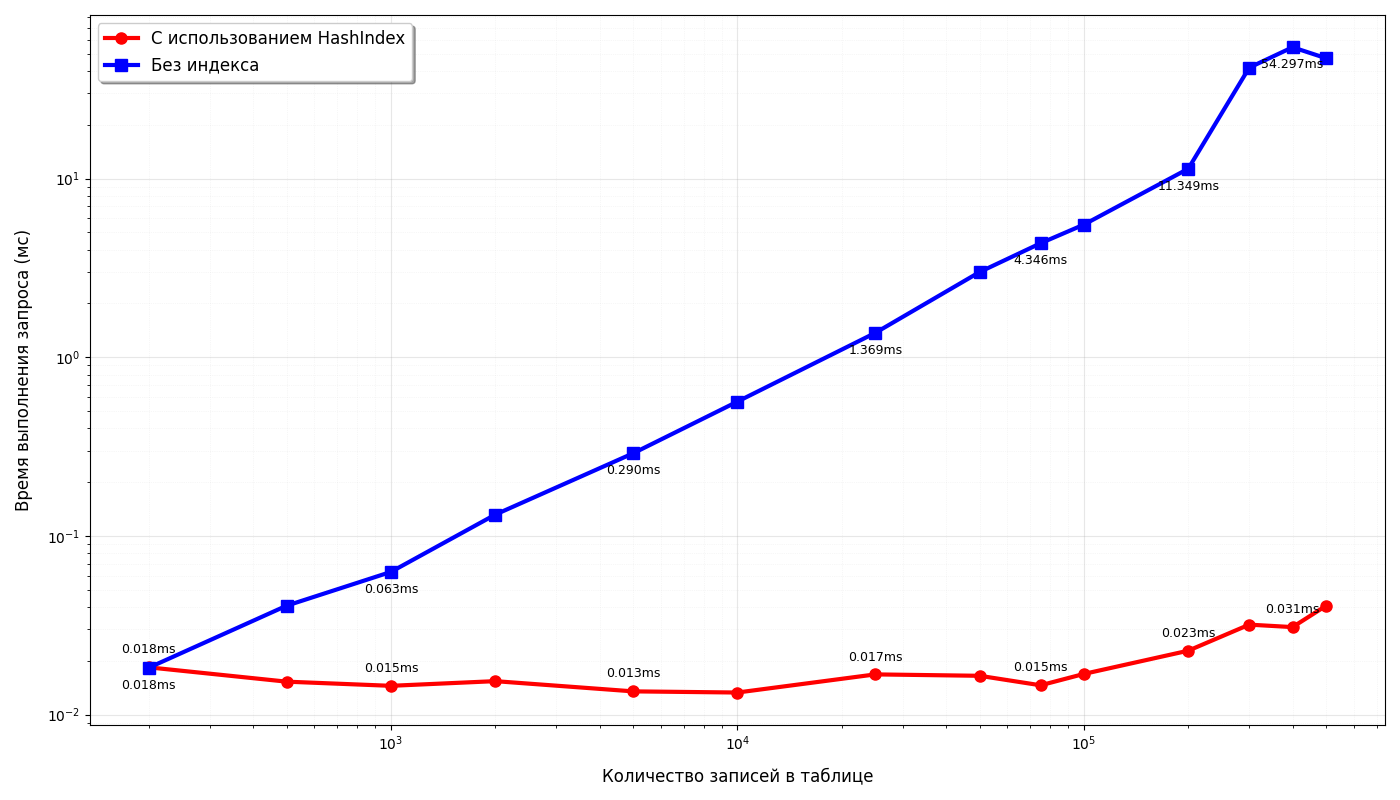
\includegraphics[width=1\textwidth]{img/hash.png}
	\caption{График времени выполнения запросов от количество записей в таблице с использованием HASH-индекса и без него}
	\label{fig:graph_hash_exe}
\end{figure}


\begin{figure}[H]
	\centering
	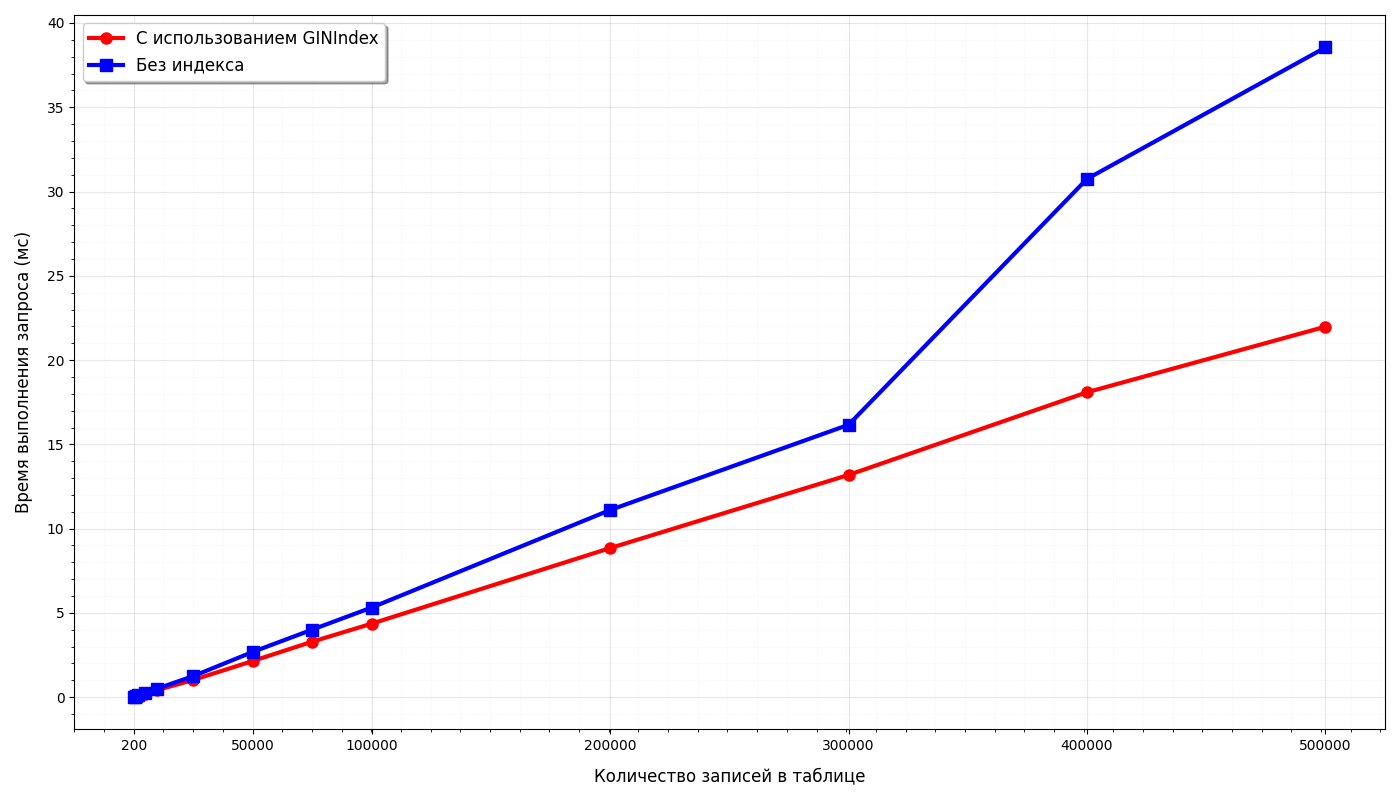
\includegraphics[width=1\textwidth]{img/gin.png}
	\caption{График времени выполнения запросов от количество записей в таблице с использованием GIN-индекса и без него}
	\label{fig:graph_gin_exe}
\end{figure}

\section{Вывод}

Использование индексов значительно уменьшает время выполнения запросов, что особенно заметно на больших таблицах.

